\chapter{Experiments}
\label{sec:experiments}

Once the kernels are implemented, we can proceed to design and run the
experiments using them. We will follow the objectives and hypotheses stated in
\cref{sec:objectives_and_hypotheses}.

\section{Common experimental setup}

\subsection{Resampling}
\label{sec:resampling}

Instead of using the double cross-test resampling used in
\cref{sec:reproducing-frenay}, we opted to use a 5\texttimes2 cross-validation
resampling method as described by
\textcite{dietterichApproximateStatisticalTests1998}.

The 5\texttimes2 cross-validation consists of doing a 50\textendash50 split of
the dataset into two sets. First, we train on the first set and test on the
second set and then we train on the second set and test on the first set. The
process is repeated 5 times, each time with a different random split. We choose
this method since it is faster than the double cross-test method requiring only
10 training processes instead of 100.

% TODO: Add figure of the 5-2 cross-validation ?

\subsection{Metrics}
\label{sec:metrics}

For the metrics on the regression problems,
we use the normalized root-mean-square error (\emph{nRMSE}),
which is a normalized version of the root-mean-square error (\emph{RMSE})
defined as follows:
\begin{equation}
    nRMSE = \sqrt{\frac{1}{n}\sum_{i=1}^n (y_i - \hat{y}_i)^2}\frac{1}{\sigma_{obs}}
\end{equation}
where $y_i$ is the observed value, $\hat{y}_i$ is the predicted value and
$\sigma_{obs}$ is the standard deviation of the observed values.

For the classification problems, we save the matrix of confusion from which we
can calculate the accuracy, precision, recall and F1 score.

Additionally, we save the number of iterations and the time needed for the
training process.

\subsection{Normalization}

In order to be able to compare the results between different datasets, an effort
was made to normalize the data and hyperparameters. To that end, the following
measures were implemented:

\begin{enumerate}
    \item Variables (including target) are standardized
    \item We use normalized root-mean-square error as our performance
          measure.
    \item The kernel itself is normalized (\cref{sec:kernel_normalization})
    \item The hyperparameter $\sigma_w$ is normalized by dividing it by the
          number of attributes of each dataset. This makes the hyperparameter
          comparable between different datasets.
\end{enumerate}

In the next paragraphs we clarify how each of these steps are implemented and
what is their effect.

\paragraph{Variable Standardization} is implemented by taking the mean and
standard derivation of each column of the training set and using it to normalize
the columns ($z_i = (x_i - \mu_i)/\sigma_i$). These values are saved as part of
the model and used again when running on the test set. This process is also
applied to the target variable.

This acts as a method of scaling the data to values that are well-behaved for
the SVM.

% TODO: all this is repeated in the implementation
\paragraph{Normalized Root-Mean-Square Error} We define the
normalized root-mean-square error (\emph{nRMSE}) as follows:
\begin{equation}
    nRMSE = \frac{RMSE}{\sigma_{obs}}
\end{equation}

\paragraph{Kernel Normalization} for a given kernel $K$, we define the
normalized kernel $\hat{K}$ as follows:
\begin{equation}
    \hat{K}(x, y) = \frac{K(x, y)}{\sqrt{K(x, x)K(y, y)}}
\end{equation}
By normalizing the kernel, we mitigate the effect of the scale of the
input variables. % TODO: Rewrite this

\paragraph{Sigma Normalization} We define the normalized sigma $\hat{\sigma}$
as follows:
\begin{equation}
    \hat{\sigma} = \frac{\sigma}{n}
\end{equation}
where $n$ is the number of attributes of the dataset. By doing so, the
hyperparameter $\sigma$ is comparable between datasets.

\subsection{Parameter grid}

For the parameter search, we tried all the combinations of values in the bounds
show in \cref{tab:paramgrid} in a $\log 10$ scale with spacing of factor of $10$
between values. For example, for $\sigma_w$ the values were
$10^{-3},\,10^{-2},\,\dots,\,10^{6}$.
% TODO: write this part so that it is more clear?

\begin{table}[H]
    \caption{Bounds of parameter grid}%
    \label{tab:paramgrid}
    \begin{tabular}{ccc}
        \toprule
        Variable      & lower     & upper  \\
        \midrule
        $\sigma_w$    & $10^{-3}$ & $10^6$ \\
        $\varepsilon$ & $10^{-5}$ & $10^1$ \\
        $C$           & $10^{-2}$ & $10^4$ \\
        \bottomrule
    \end{tabular}
\end{table}

\section{Reproducing the results of \texorpdfstring{\citeauthor{frenayParameterinsensitiveKernelExtreme2011}}{Frénay and Verleysen}}
\label{sec:reproducing-frenay}

The first objective is to reproduce the results obtained by
\textcite{frenayParameterinsensitiveKernelExtreme2011}, which will help validate
our implementation of the arc sine kernel, ensure that our experimental setup is
correct and to have a baseline to compare our results with. This also serves as
a peer review of their results.

\subsection{Considerations on the resampling method}

In the paper, \citeauthor{frenayParameterinsensitiveKernelExtreme2011} use a
double cross-test resampling method which is illustrated in
\cref{fig:frenay-cross-test}. First, they perform a 10-fold cross validation,
where the 9 folds of the training set are then used on a second 10-fold cross
validation to determine the best hyperparameters. This means that there are 100
training processes in total.

\begin{figure}[H]
    \begin{tikzpicture}[
		scale=0.66,
		every node/.style={font=\footnotesize},
	]
	% Draw main rectangle
	\def\nfolds{10}
	\pgfmathsetmacro{\trainfolds}{\nfolds-1}
	\pgfmathsetmacro{\splits}{\nfolds-2}
	\def\heightmult{0.5}

	\newcommand{\fold}[5]{%
		\draw[#2] #1 rectangle ($#1+(\heightmult*\trainfolds,1)$);
		% fill with pattern
		\filldraw[#3] ($#1+(\heightmult*\trainfolds,0)$) rectangle ($#1+(\heightmult*\nfolds,1)$);

		\draw ($#1+(\heightmult*\trainfolds/2,0)$) node[below,name=below-#5] {training set};
		\draw ($#1+(\heightmult*\nfolds,0.5)$) node[right,name=right-#5] {#4 set};

		% Draw vertical dashed lines for fold divisions
		\foreach \x in {1,...,\splits}{
				\draw ($#1+(\heightmult*\x,0)$) -- ($#1+({\heightmult*\x},1)$);
			}
	}

	\def\coltest{wong_blue}
	\def\colvali{wong_orange}

	\fill[shading=axis,top color=\coltest!40,bottom color=\colvali!40] (0,0) -- (\heightmult*\trainfolds,0) -- (\heightmult*\nfolds,-1) -- (0,-1) -- cycle;

	\fold{(0,0)}{fill=\coltest}{pattern=north east lines, pattern color=\coltest}{test}{test1}
	\fold{(0,-2)}{fill=\colvali}{pattern=north west lines,pattern color=\colvali}{validation}{val1}

	\draw[->] (0,0) -- (0,-1);
	\draw[->] (\heightmult*\trainfolds,0) -- (\heightmult*\nfolds,-1);

	% title above bounding box
	% \draw (current bounding box.north) node[above] {\textbf{Step 1: folding}};

	\fold{(9,0)}{fill=\colvali}{pattern=north west lines,pattern color=\colvali}{validation}{val2}

	\draw (right-val1.east -| below-val2.south) node[name=meta-parameters] {meta-parameters};
	\coordinate (a) at ($(meta-parameters)!.5!(below-val2)$);
	\node[name=model] at (a -| right-val2) {model};

	\coordinate (vm) at ($(model)!.5!(right-val2)$);
	\node[name=valerr] at ($(vm)+(5,0)$) {validation error};

	\coordinate (mm) at ($(meta-parameters.east |- model.west)!0.5!(model.west)$);
	\draw (below-val2.east) -| (mm);
	\draw (meta-parameters.east) -| (mm);
	\draw[->] (mm) -- (model);

	\coordinate (vvm) at ($(right-val2.east |- valerr.west)!0.5!(valerr.west)$);
	\draw (right-val2.east) -| (vvm);
	\draw (model.east) -| (vvm);
	\draw[->] (vvm) -- (valerr);

	% step 3

	\coordinate (step3) at (5,-5);
	\fold{(step3)}{fill=\coltest}{pattern=north east lines,pattern color=\coltest}{test}{test3}

	\draw ($(below-test3.south)+(0,-1)$) node[name=best-meta-parameters,text width=3cm,align=center]
	{best meta-parameters selected by cross-validation};

	\coordinate (b) at ($(best-meta-parameters)!.5!(below-test3)$);
	\node[name=model3] at ($(b -| right-test3)+(1,0)$) {model};

	\coordinate (vm3) at ($(model3)!.5!(right-test3)$);
	\node[name=testerr] at ($(vm3)+(5,0)$) {test error};

	\coordinate (mm3) at ($(best-meta-parameters.east |- model3.west)!0.5!(model3.west)$);
	\draw (below-test3.east) -| (mm3);
	\draw (best-meta-parameters.east) -| (mm3);
	\draw[->] (mm3) -- (model3);

	\coordinate (vvm3) at ($(right-test3.east |- testerr.west)!0.5!(testerr.west)$);
	\draw (right-test3.east) -| (vvm3);
	\draw (model3.east) -| (vvm3);
	\draw[->] (vvm3) -- (testerr);

	\coordinate (shift) at (0,1.5);
	\draw ($(0,0)+(shift)$) node[right] {\textbf{Step 1: folding}};
	\draw ($(9,0)+(shift)$) node[right] {\textbf{Step 2: meta-parameters selection on validation set}};
	\draw ($(step3)+(shift)$) node[right] {\textbf{Step 3: model assessment on test set}};

	% \draw ($(9,0)!0.5!(valerr.east) + (0,1.1)$) node[above] {\textbf{Step 2: meta-parameters selection on validation set}};

	% \draw ($(step3)!0.5!(step3 -| testerr.east) + (0,1)$) node[above] {\textbf{Step 3: model assessment on test set}};

\end{tikzpicture}

    \caption{Illustration of the cross-test method from \cite{frenayParameterinsensitiveKernelExtreme2011}}
    \label{fig:frenay-cross-test}
\end{figure}

As mentioned in \cref{sec:resampling}, we opted to use a 5\texttimes2 cross
which sacrifices part of the statistical power of their method in favor of
speed. This decision was made since 5\texttimes2 should be enough to get a
reasonable estimate of the performance and verify that the results are
consistent with the paper without requiring a lot of computational power.

\subsection{Results for the arc sine kernel on the Frenay datasets}

% TODO: bands for std or no bands, if not, make sure that the explaination below
% is clear.
\begin{important}
    Remove STD bands?
\end{important}
\begin{figure}[H]
    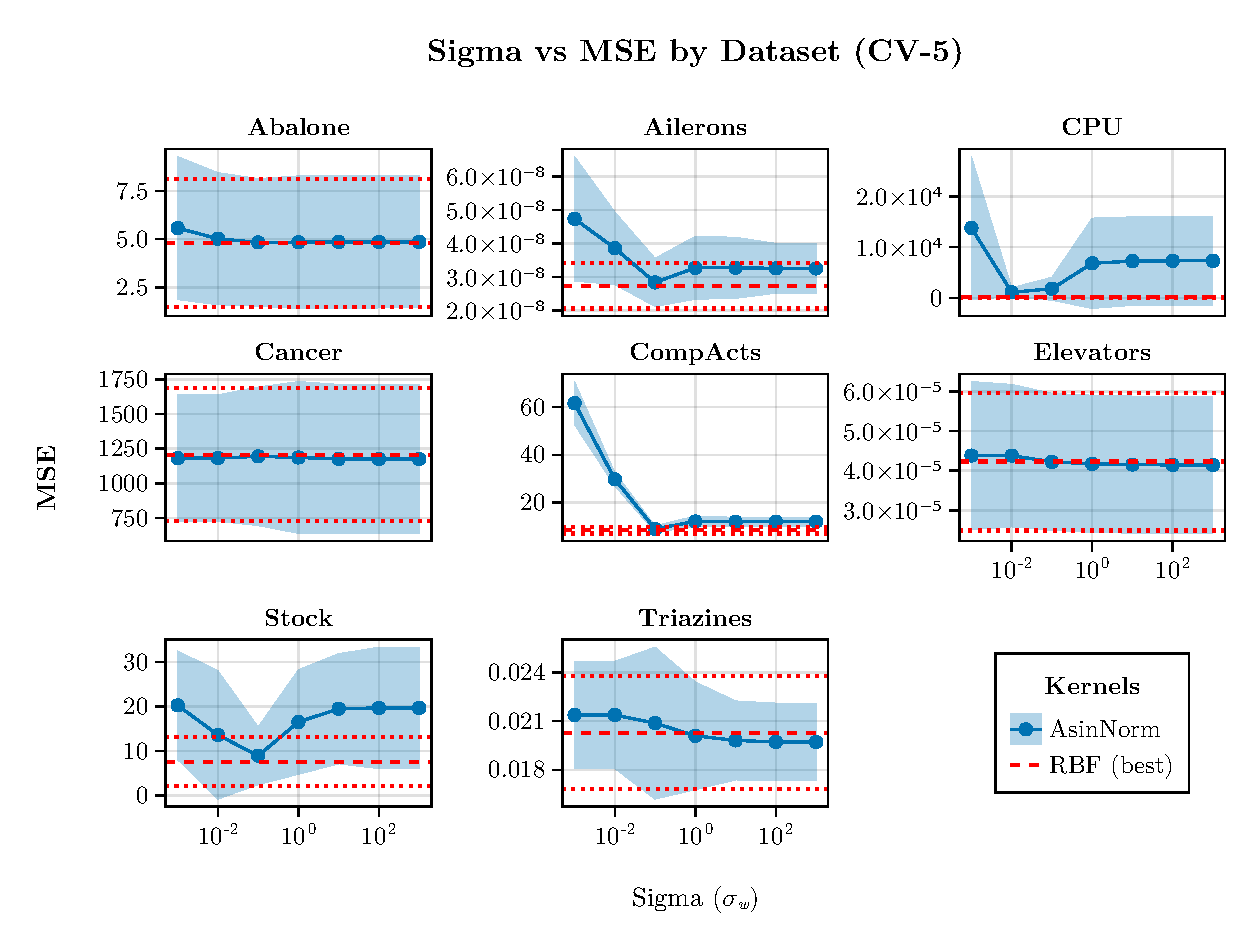
\includegraphics[width=\textwidth]{plots/MSE_frenay}
    \caption{MSE results on datasets from \cite{frenayParameterinsensitiveKernelExtreme2011}}
    \label{fig:mse-frenay}
\end{figure}

\Cref{fig:mse-frenay} shows the results of the arc-sine
kernel~(normalized and non-normalized) on the same datasets used by \textcite{frenayParameterinsensitiveKernelExtreme2011}. The shading corresponds to the standard deviation when averaging the
cross-validation results.

The results are consistent with the results obtained by \citeauthor{frenayParameterinsensitiveKernelExtreme2011}.
Except for the \texttt{CPU} dataset, which in the original paper is reported to
not be significantly different from the RBF kernel for $\sigma_w > 0.1$. In
our results, the optimal value of $\sigma_w$ is $0.01$ which is indeed not
significantly different from the RBF kernel, but once we increase $\sigma_w$,
the performance drops significantly and converges to a much higher value than
expected. This may be due to the fact that the \texttt{CPU} dataset is very
small and thus the difference in our resampling method is more noticeable.

What we can conclude however is that both the normalized and non-normalized
arc-sine kernel do seem to be insensitive to the value of $\sigma_w$ for
$\sigma_w > 0.1$.

\begin{figure}[H]
    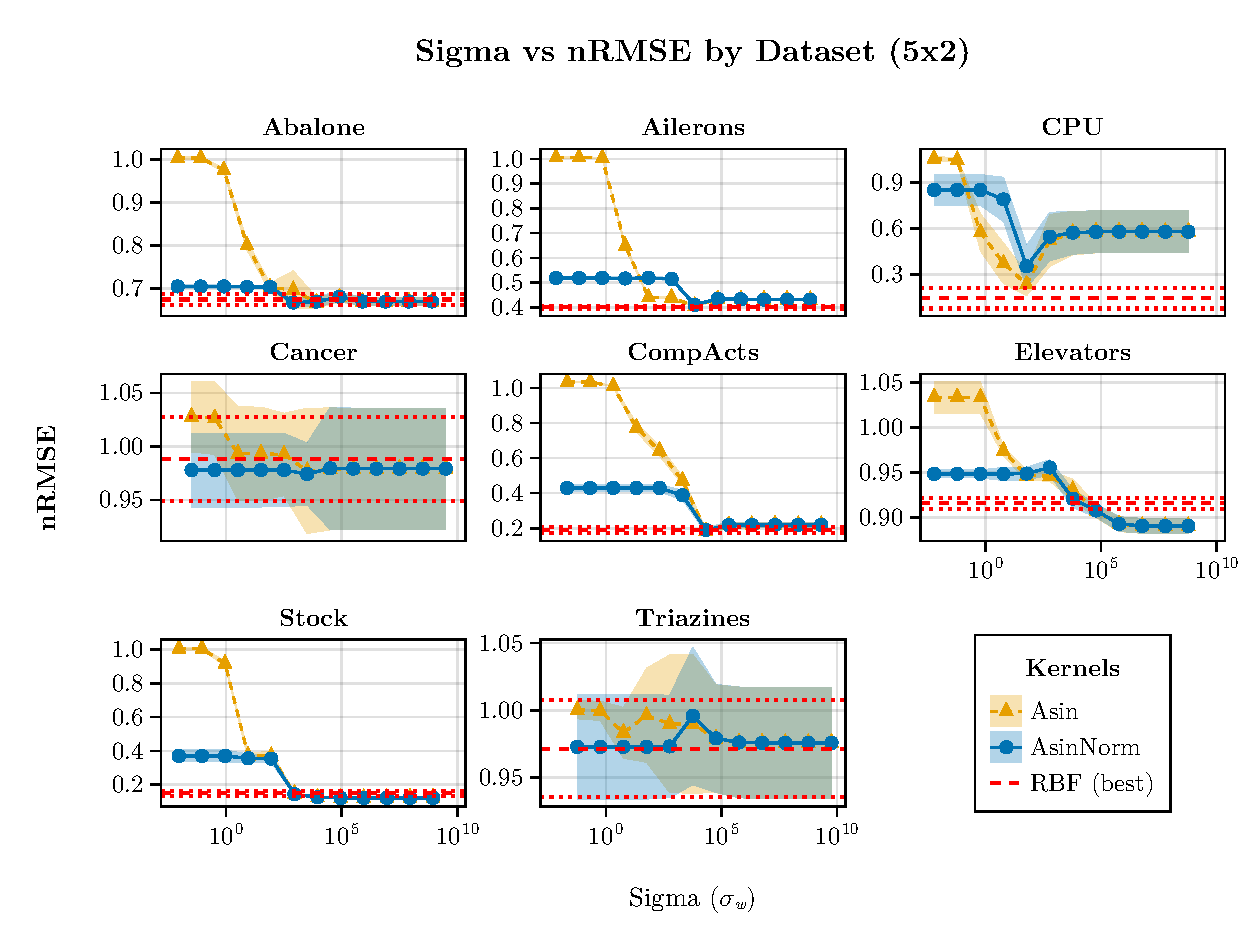
\includegraphics{plots/nRMSE_frenay_scaled}
    \caption{nRMSE results on datasets from \cite{frenayParameterinsensitiveKernelExtreme2011} with
        scaled $\sigma_w$}%
    \label{fig:nrmse-frenay-scaled}
\end{figure}

\Cref{fig:nrmse-frenay-scaled} shows the results of the arc-sine kernel using
\emph{nRMSE} as the performance measure and with $\sigma_w$ scaled. These allow
us to compare the results between datasets.

\begin{cnote}
    Add copy of the table of Frénay and Verleysen along with the equivalent
    table for our results?

    The table is quite dense, so putting them side by side my be too much.

    Figure out what is the most relevant information to show, rest in the
    appendix
\end{cnote}

\subsection{Results for the arc cosine kernel on the Frenay datasets}

\Cref{fig:nrmse-acos-frenay-scaled} shows the results when using the arc cosine kernels
with $n=0,1,2$ on the Frenay datasets.

\begin{figure}[H]
    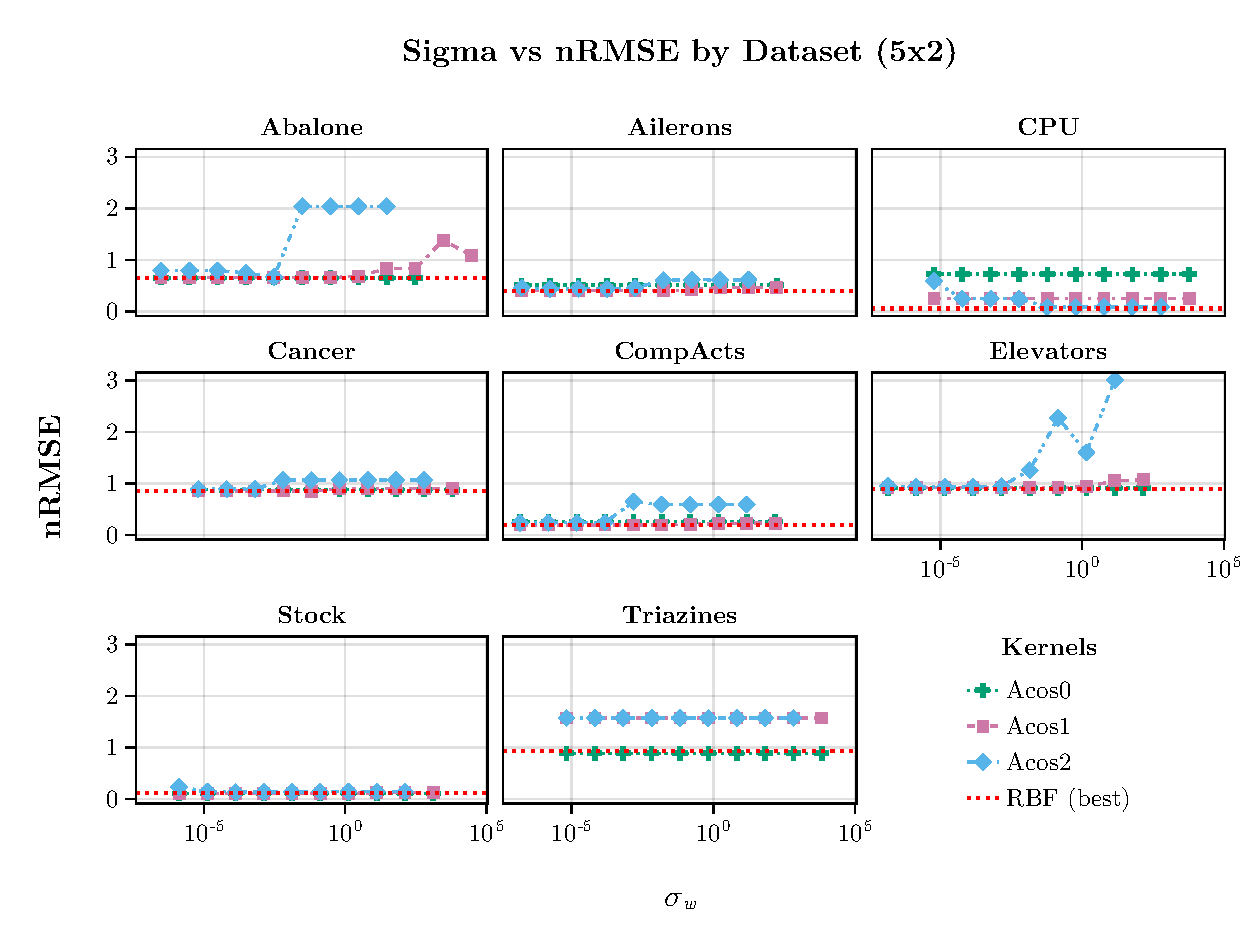
\includegraphics{plots/nRMSE_acos_frenay_scaled}
    \caption{nRMSE results on datasets from \cite{frenayParameterinsensitiveKernelExtreme2011} with
        scaled $\sigma_w$ using Arc cosine kernel}%
    \label{fig:nrmse-acos-frenay-scaled}
\end{figure}

\begin{cnote}
    Arc cosine kernel for n=2 is too slow (specially when $cost>1000$)
    I have removed it, but ideally we run it with a smaller parameter grid.
    Should be addressed either way.
\end{cnote}


\section{Execution time and number of iterations}%
\label{sec:execution-time-and-number-of-iterations}

\begin{figure}[H]
    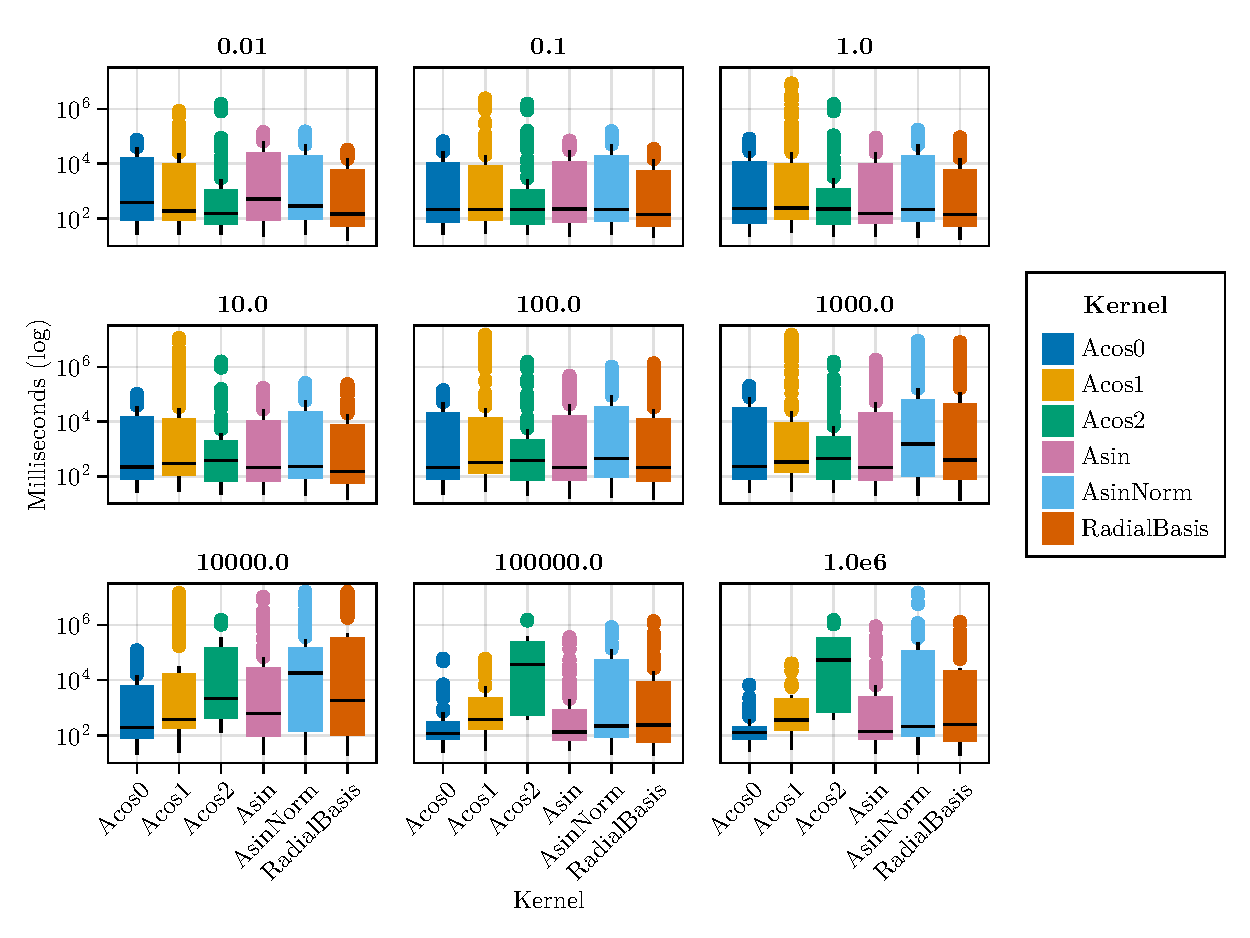
\includegraphics{plots/execution_log}
    \caption{Execution time of the different kernels (log scale) Changing the cost
        parameter}%
    \label{fig:execution-log}
\end{figure}

\Cref{fig:execution-log} shows boxplots of the execution times of the different
kernels for across all datasets. The title above each subplot indicates the
value of the cost parameter. As we can see, increasing the cost parameter
increases the execution time of the SVM. This effect is more noticeable for the
kernels with more complex computations, such as the normalized arc-sine kernel
and specially the arc-cosine kernels with $n=1$ and $n=2$.

\begin{cnote}
    These values of the cost are too high.
    In the other plots, we use $10^4$ as the upper bound.
    We should probably remove the bottom row altogether.

    Also, add cost=... to the subplot titles
\end{cnote}

\begin{figure}[H]
    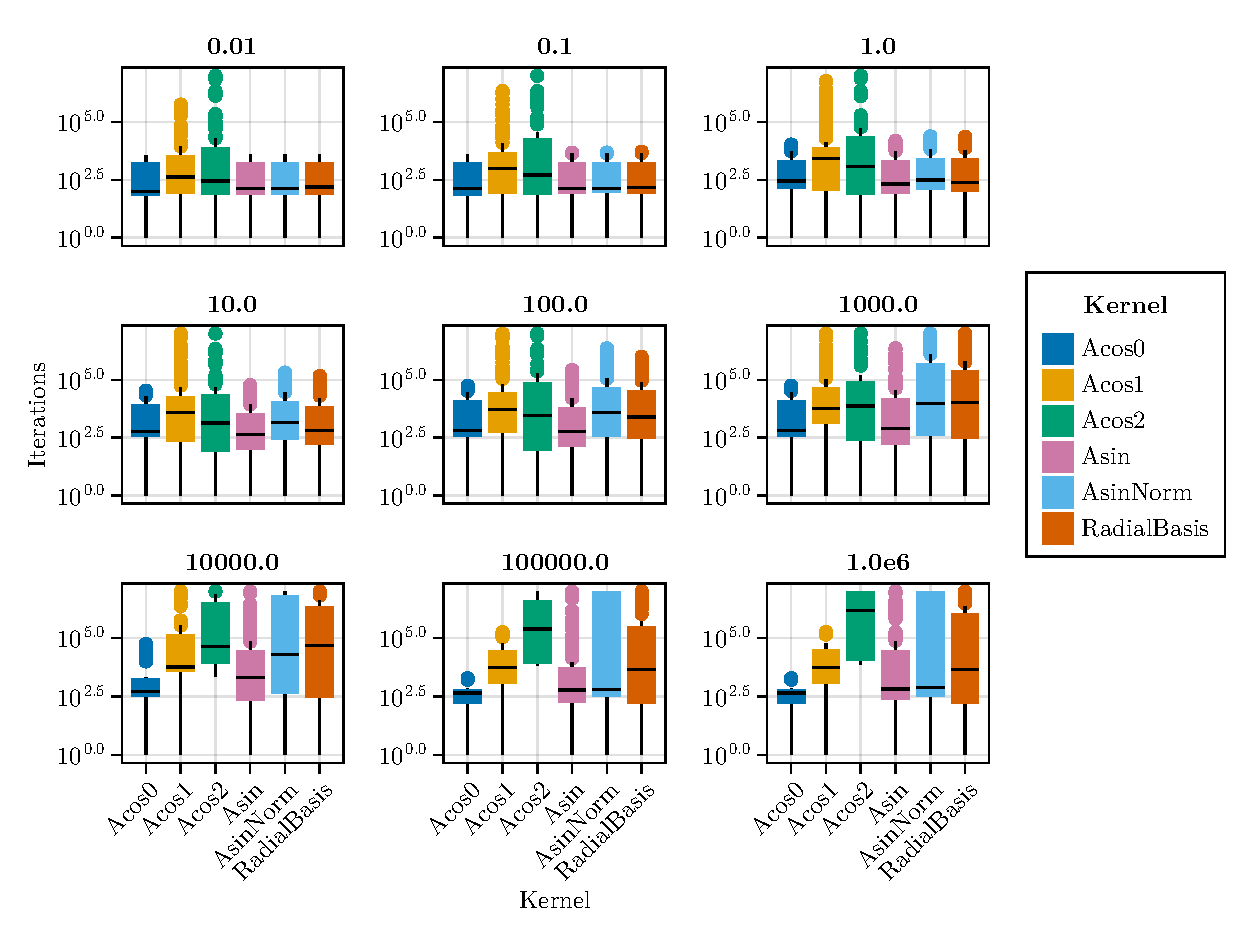
\includegraphics{plots/iter_log}
    \caption{Iterations needed for different kernels (log scale) Changing the cost
        parameter}
\end{figure}

\begin{cnote}
    Why asin-norm has more iterations than asin in average?
\end{cnote}

\section{Comparing the performance of the kernels with different datasets}%
\sectionmark{Comparing performance}

\subsection{Delve (Bank and PumaDyn) dataset families}

The Delve datasets are a collection of datasets used in the Delve project,
among them are the Bank and PumaDyn datasets. There are 8 variations of
these datasets, which come from the combination of these properties%
\footnote{\url{https://www.cs.toronto.edu/~delve/data/families.html}}:
\begin{description}
    \item[Attributes] 32 or 8
    \item[Linearity] Fairly linear or Nonlinear
    \item[Noise] High or Low.
\end{description}

% We refer to a specific combination as \texttt{Bank32fh}, which corresponds to
% the Bank dataset with 32 attributes, \textbf{f}airly linear and \textbf{h}igh
% noise.

\subsubsection{Bank}

\begin{figure}[H]
    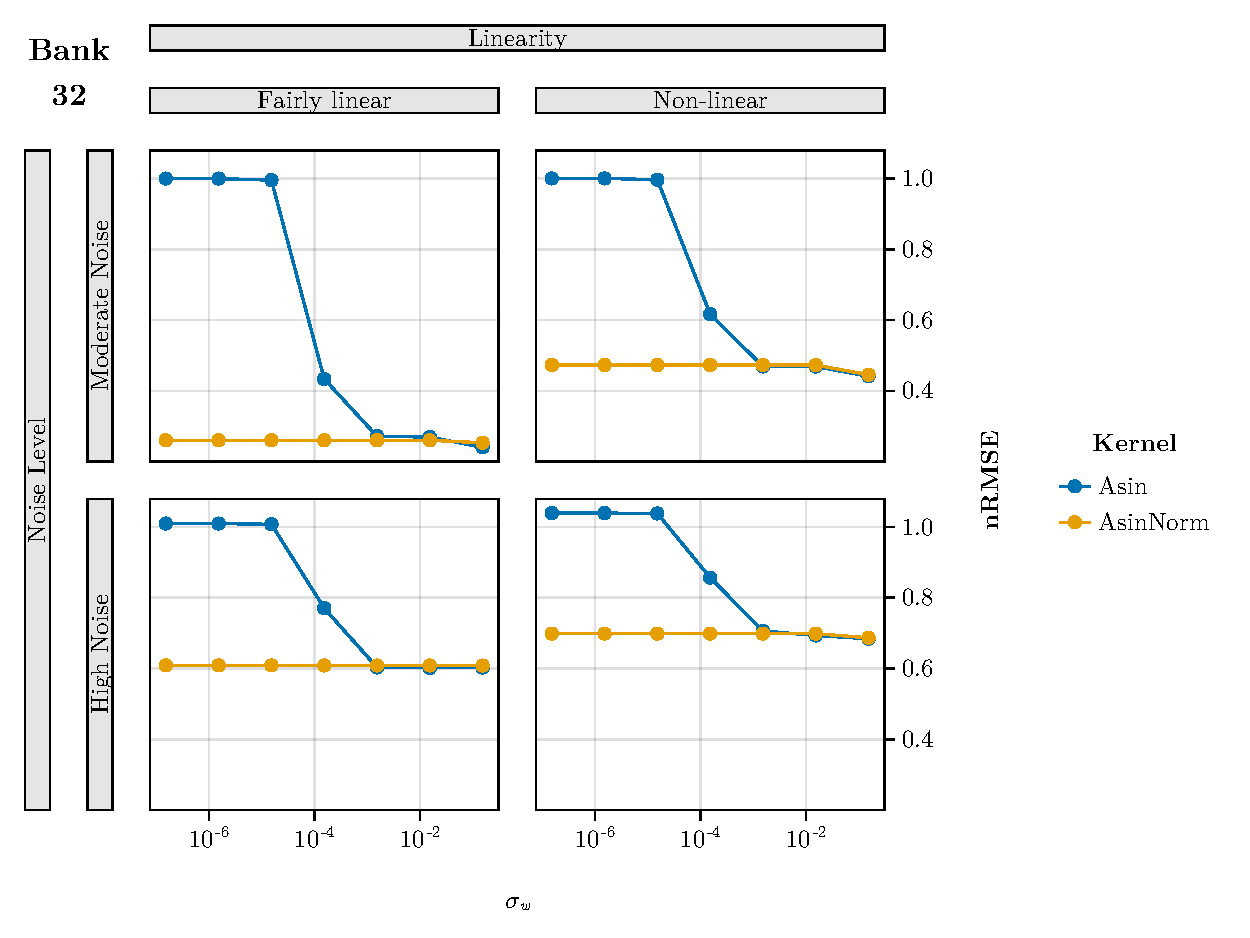
\includegraphics[width=0.7\textwidth]{plots/nRMSE_delve_bank_32_scaled}
    \caption{nRMSE results on Delve Bank32 dataset with $\sigma_w$ scaled}
    \label{fig:nrmse-delve-bank-32-scaled}
\end{figure}

\begin{figure}[H]
    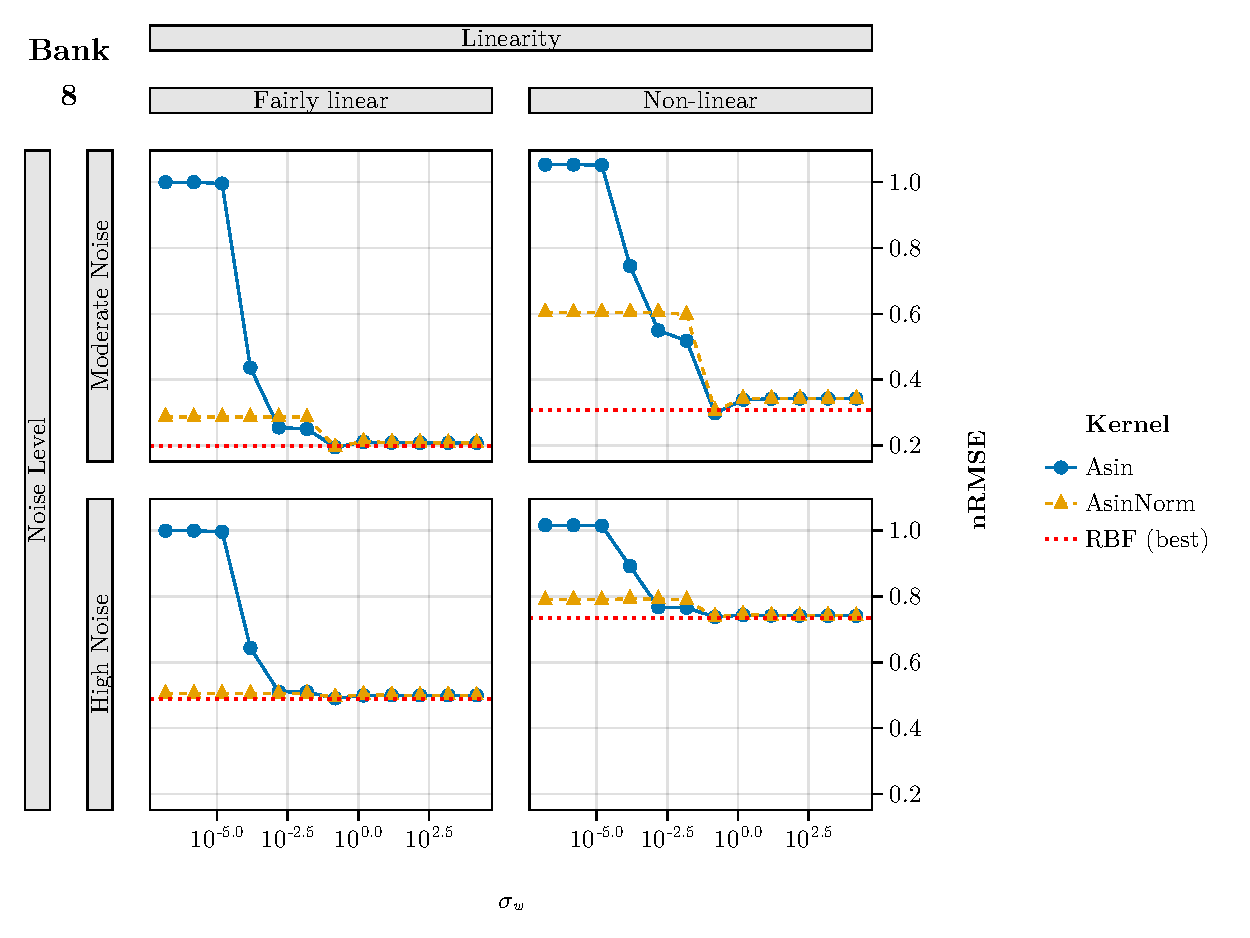
\includegraphics[width=0.7\textwidth]{plots/nRMSE_delve_bank_8_scaled}
    \caption{nRMSE results on Delve Bank8 dataset with $\sigma_w$ scaled}
    \label{fig:nrmse-delve-bank-8-scaled}
\end{figure}

\subsubsection{Pumadyn}

\begin{figure}[H]
    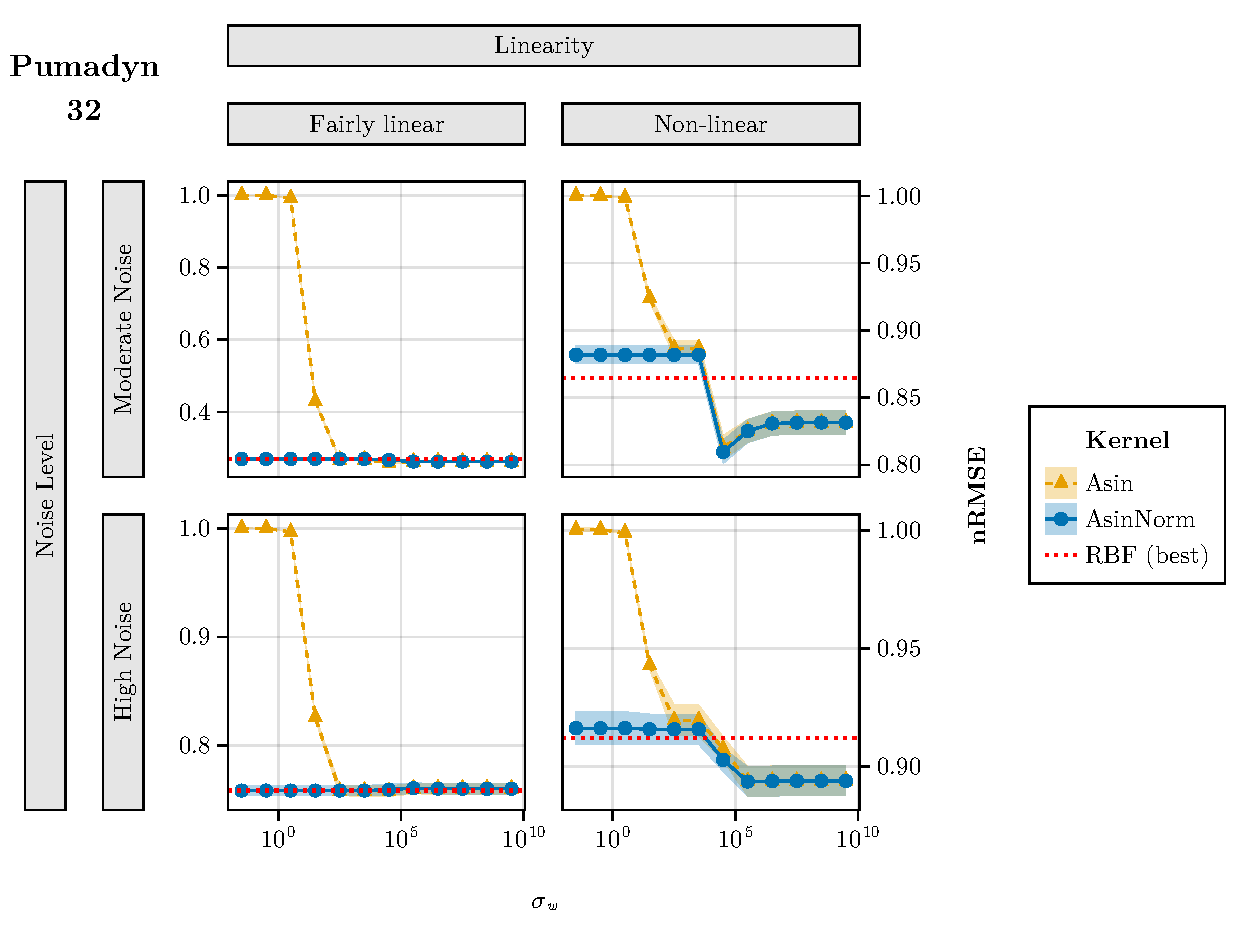
\includegraphics[width=0.7\textwidth]{plots/nRMSE_delve_pumadyn_32_scaled}
    \caption{nRMSE results on Delve PumaDyn32 dataset with $\sigma_w$ scaled}
    \label{fig:nrmse-delve-pumadyn-32-scaled}
\end{figure}

\begin{figure}[H]
    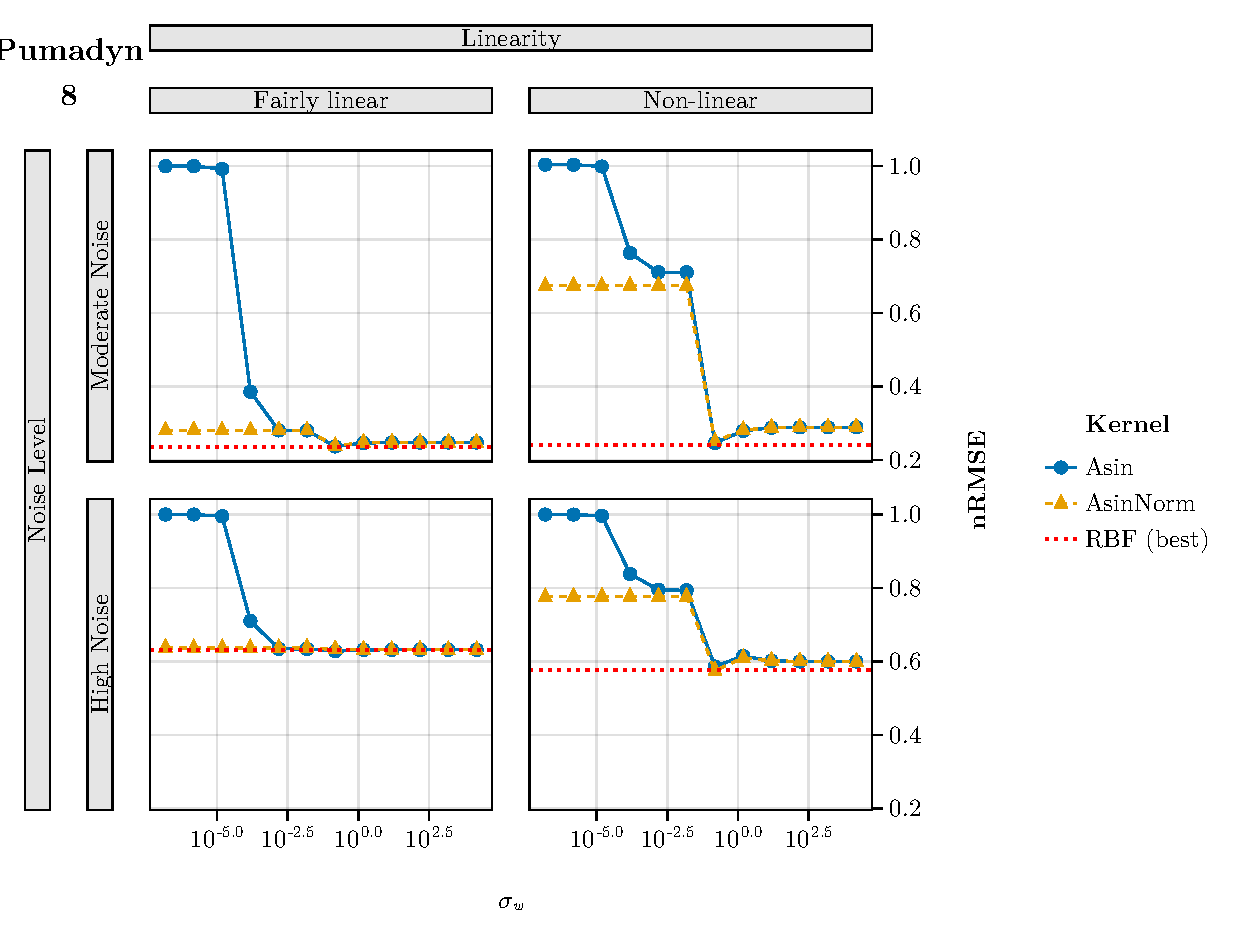
\includegraphics[width=0.7\textwidth]{plots/nRMSE_delve_pumadyn_8_scaled}
    \caption{nRMSE results on Delve PumaDyn8 dataset with $\sigma_w$ scaled}
    \label{fig:nrmse-delve-pumadyn-8-scaled}
\end{figure}

\Cref{fig:nrmse-delve-bank-32-scaled,fig:nrmse-delve-bank-8-scaled,fig:nrmse-delve-pumadyn-32-scaled,fig:nrmse-delve-pumadyn-8-scaled}
show the results obtained on the different datasets in the Band and PumaDyn
families. We can see that the arc-sine kernels do converge when $\sigma_w > 1$.
In the fairly linear datasets, there is not much difference to the RBF kernel,
but in the non-linear there are situations where there is a noticeable
difference. In particular, we see a similar behaviour to the one observed in the
CPU dataset, in which there is a value of $\sigma_w$ that is \emph{optimal} (in
the sense that is not significantly different from the RBF kernel) but
increasing $\sigma_w$ does worsen the performance. This seems to contradict the
theory that there is a threshold $t$ for which increasing $\sigma_w > t$ does
not affect the result and this result is optimal.

It seems that the linearity of the dataset determines whether the arc-sine
kernel performs as the state-of-the-art RBF kernel or not when $\sigma_w$ is
large. This is an interesting result, since we may be able to use meta-learning
to determine if a dataset is a good candidate for the arc-sine kernel or not.

% TODO: can we really draw conclusions from this?

\subsection{Delve (Bank and PumaDyn) dataset using arc cosine}

% TODO: every result with acos is weird

\subsubsection{Bank}

\begin{figure}[H]
    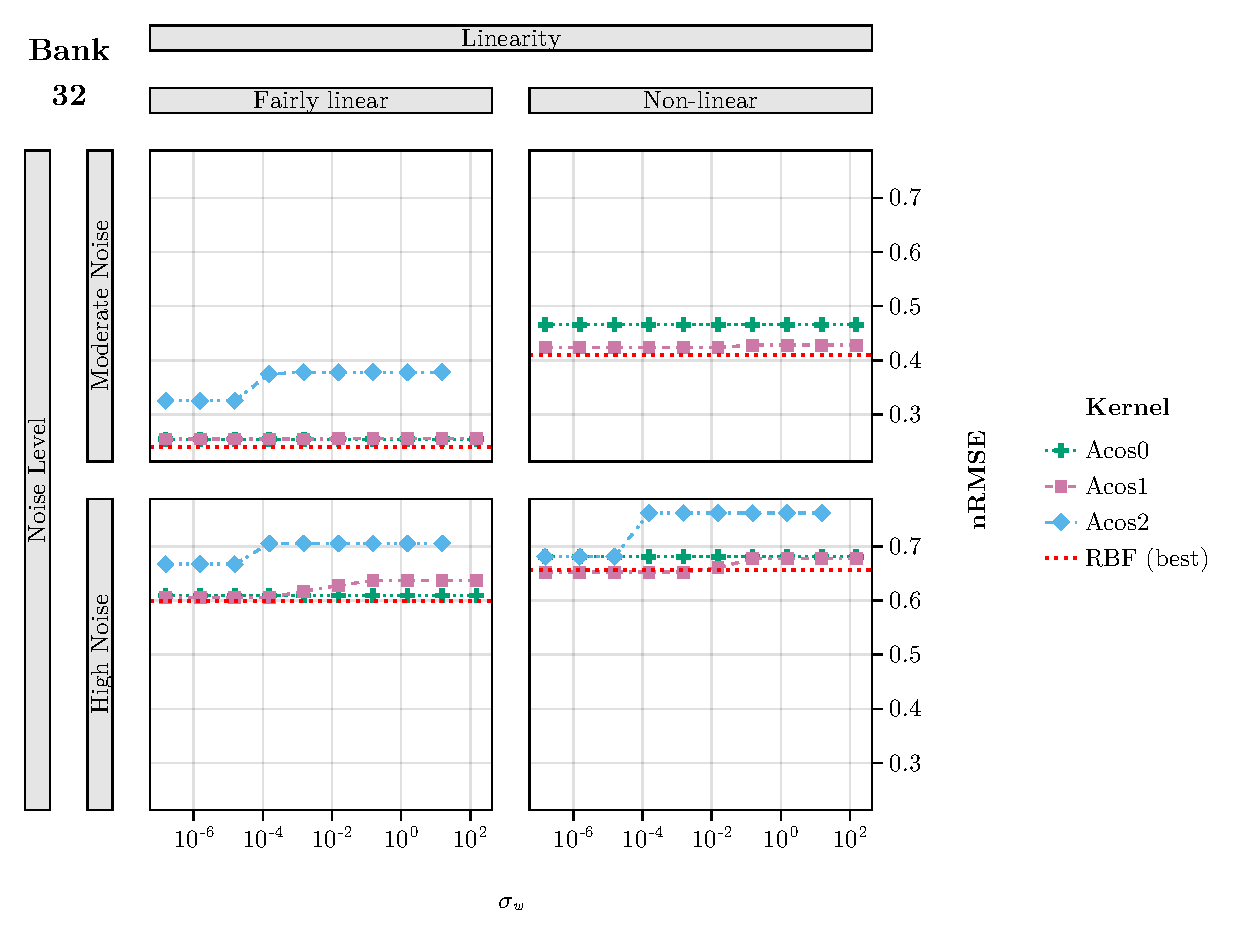
\includegraphics[width=0.7\textwidth]{plots/nRMSE_acos_delve_bank_32_scaled}
    \caption{nRMSE results on Delve Bank32 dataset with $\sigma_w$ scaled}
    \label{fig:nrmse-acos-delve-bank-32-scaled}
\end{figure}

\begin{figure}[H]
    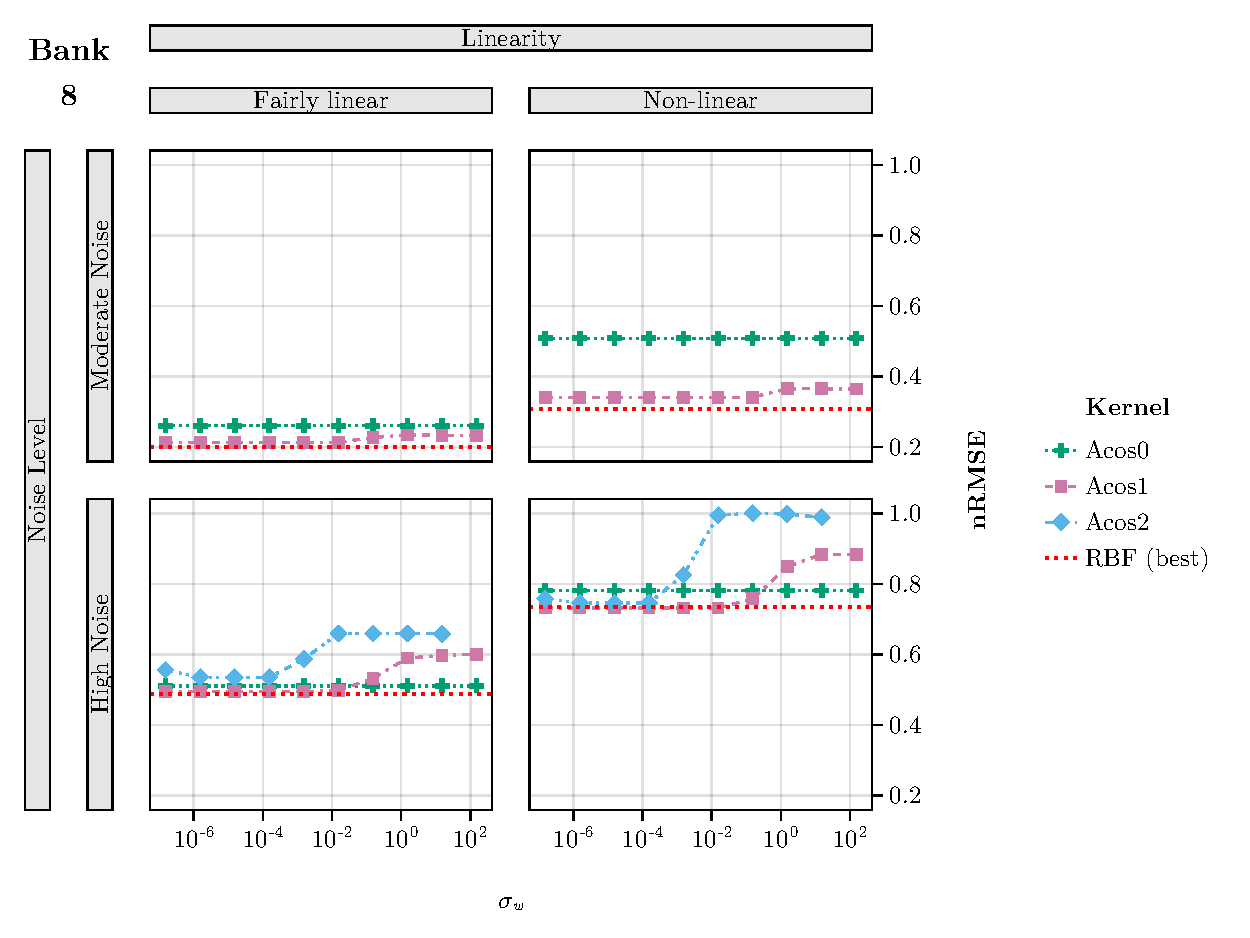
\includegraphics[width=0.7\textwidth]{plots/nRMSE_acos_delve_bank_8_scaled}
    \caption{nRMSE results on Delve Bank8 dataset with $\sigma_w$ scaled}
    \label{fig:nrmse-acos-delve-bank-8-scaled}
\end{figure}

\subsubsection{Pumadyn}

\begin{figure}[H]
    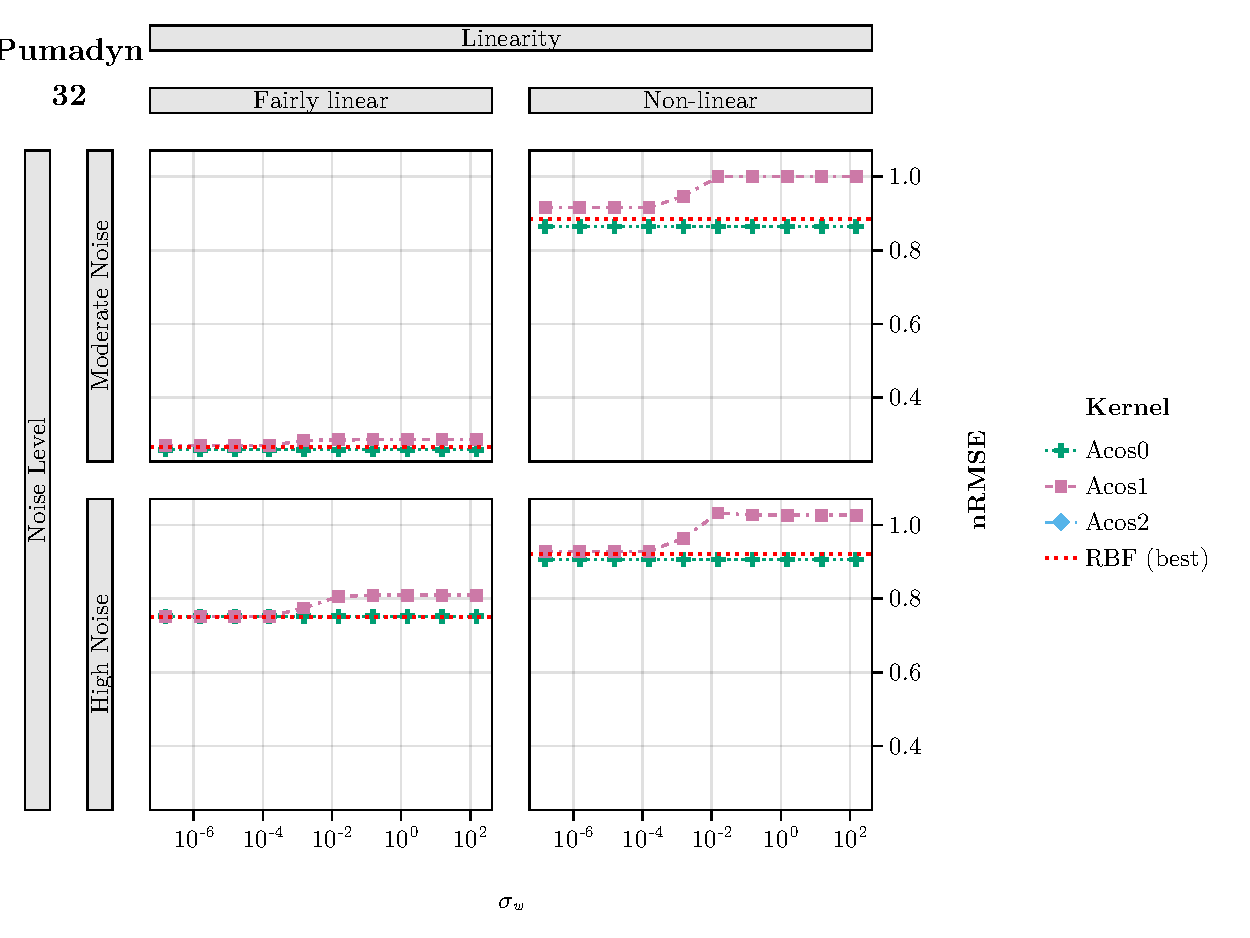
\includegraphics[width=0.7\textwidth]{plots/nRMSE_acos_delve_pumadyn_32_scaled}
    \caption{nRMSE results on Delve PumaDyn32 dataset with $\sigma_w$ scaled}
    \label{fig:nrmse-acos-delve-pumadyn-32-scaled}
\end{figure}

\begin{figure}[H]
    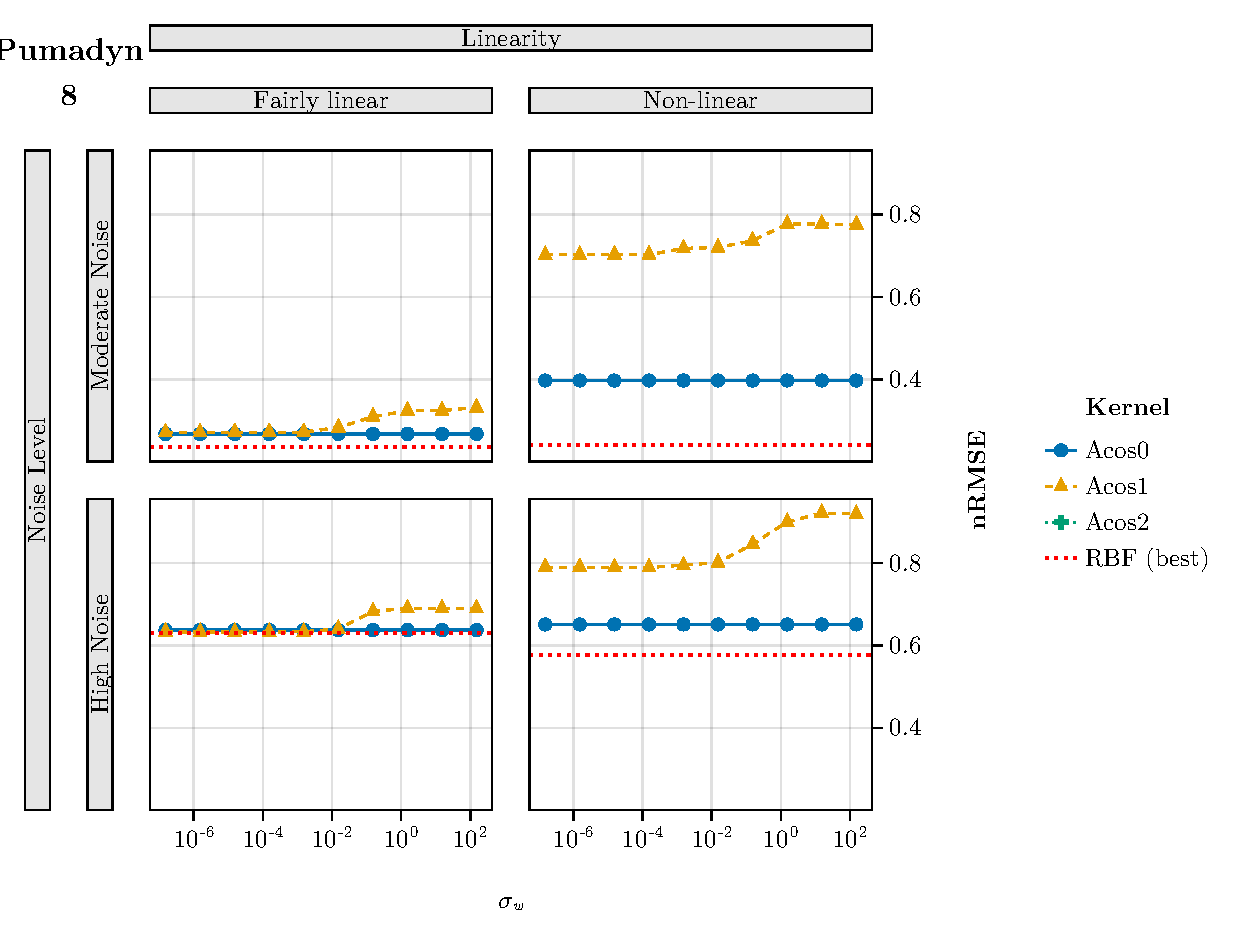
\includegraphics[width=0.7\textwidth]{plots/nRMSE_acos_delve_pumadyn_8_scaled}
    \caption{nRMSE results on Delve PumaDyn8 dataset with $\sigma_w$ scaled}
    \label{fig:nrmse-acos-delve-pumadyn-8-scaled}
\end{figure}

\begin{figure}[H]
    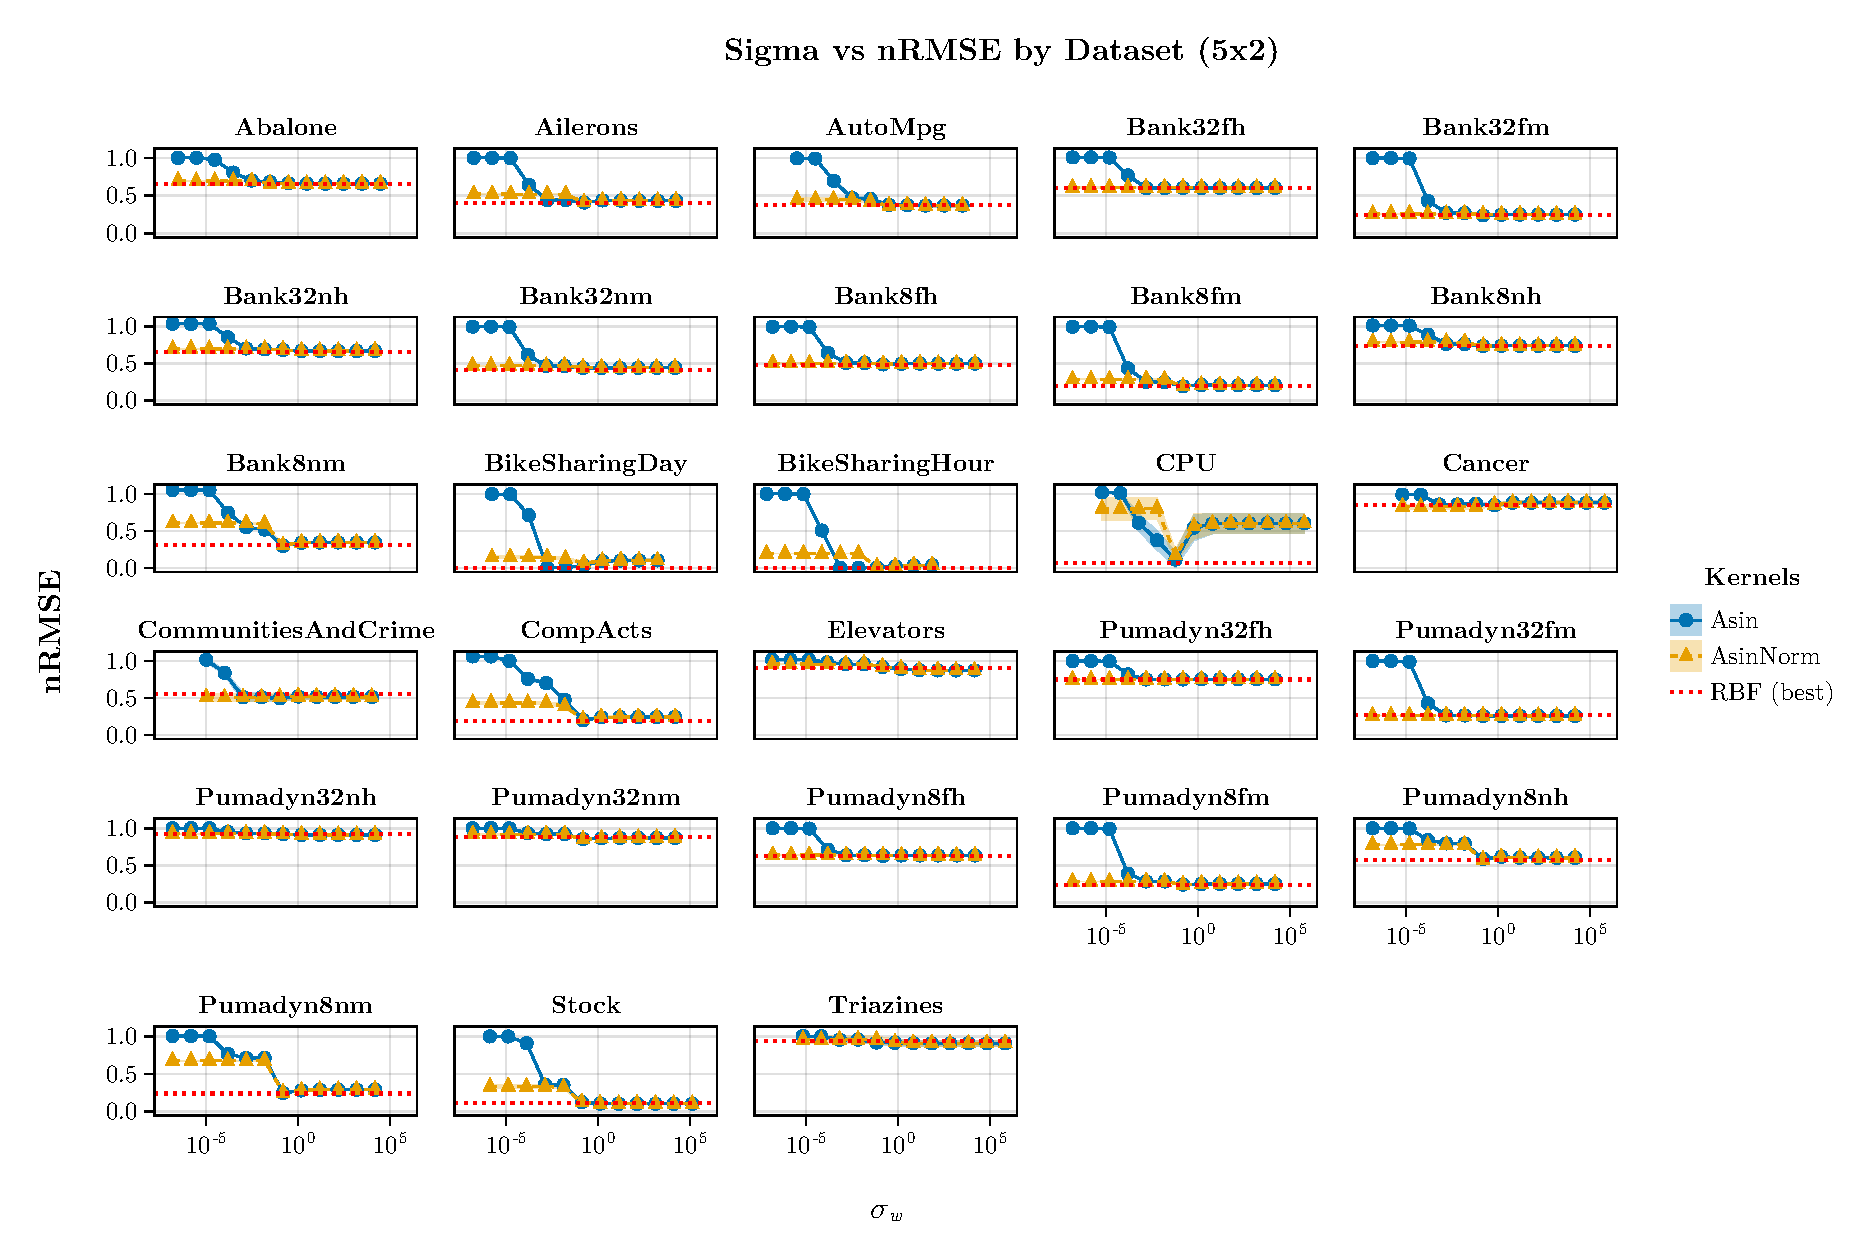
\includegraphics[width=0.9\textwidth]{plots/nRMSE_all_scaled}
    \caption{nRMSE results on all datasets with $\sigma_w$ scaled}
    \label{fig:nrmse-all-scaled}
\end{figure}

% TODO: no em convenc el titol
\subsection{Relation between the hyperparameters of the arc-sine and RBF kernels}

% TODO: t statistic instead of nRMSE?

% TODO: cite
From the results obtained in the previous section, we can see that the
arc-sine kernel (both normalized and non-normalized) seems to be able
to achieve similar performance to the RBF kernel when $\sigma_w$.

To further explore this, we can compare the relationship between the hyperparameter
$\sigma_w$ of the arc-sine kernel and the hyperparameter $\gamma$ of the RBF
kernel.

% TODO: explain this properly
% \begin{equation*}
%     \Delta_{ij} = nRMSE_i - nRMSE_j
% \end{equation*}
% Where $nRMSE_i$ 

\Cref{fig:heatmaps-rbf-asinnorm} shows the difference between the nRMSE of the
RBF and the normalized arc-sine kernel.

Positive values (in blue) indicate that for that
combination of $\sigma_w$ and $\gamma$, the normalized arc-sine kernel
outperforms the RBF kernel.
Negative values (in red) indicate that the RBF
kernel performs better than the normalized arc-sine kernel.
The darker the color, the bigger the difference.

We can observe 3 different behaviours:
\begin{itemize}
    \item The difference between the RBF and normalized arc-sine
          kernels is barely noticeable: \texttt{Cancer}, \texttt{LiverDisorders},
          \texttt{Triazines}, \dots. Looking at the results from the previous
          sections, these are \emph{hard} datasets, in the sense that the
          \emph{nRMSE} obtained by both the RBF and other kernels is high (>0.8).

    \item There is no clear effect of $\sigma_w$ on the
          performance of the normalized arc-sine kernel: \texttt{Bank32fh},
          \texttt{Bank32fm}, \texttt{CommunitiesAndCrime}, \texttt{Pumadyn32fm}, \dots

    \item There is threshold for $\sigma_w$ where the normalized
          arc-sine kernel goes from performing worse than the RBF kernel to
          performing equally or better than RBF.
\end{itemize}

% TODO: explain better
Again, the \texttt{CPU} dataset exhibits a different behaviour where for
$\sigma_w=0.1$ it is able to match the performance of the RBF kernel, but
all the others it's significantly worse.

\begin{figure}[H]
    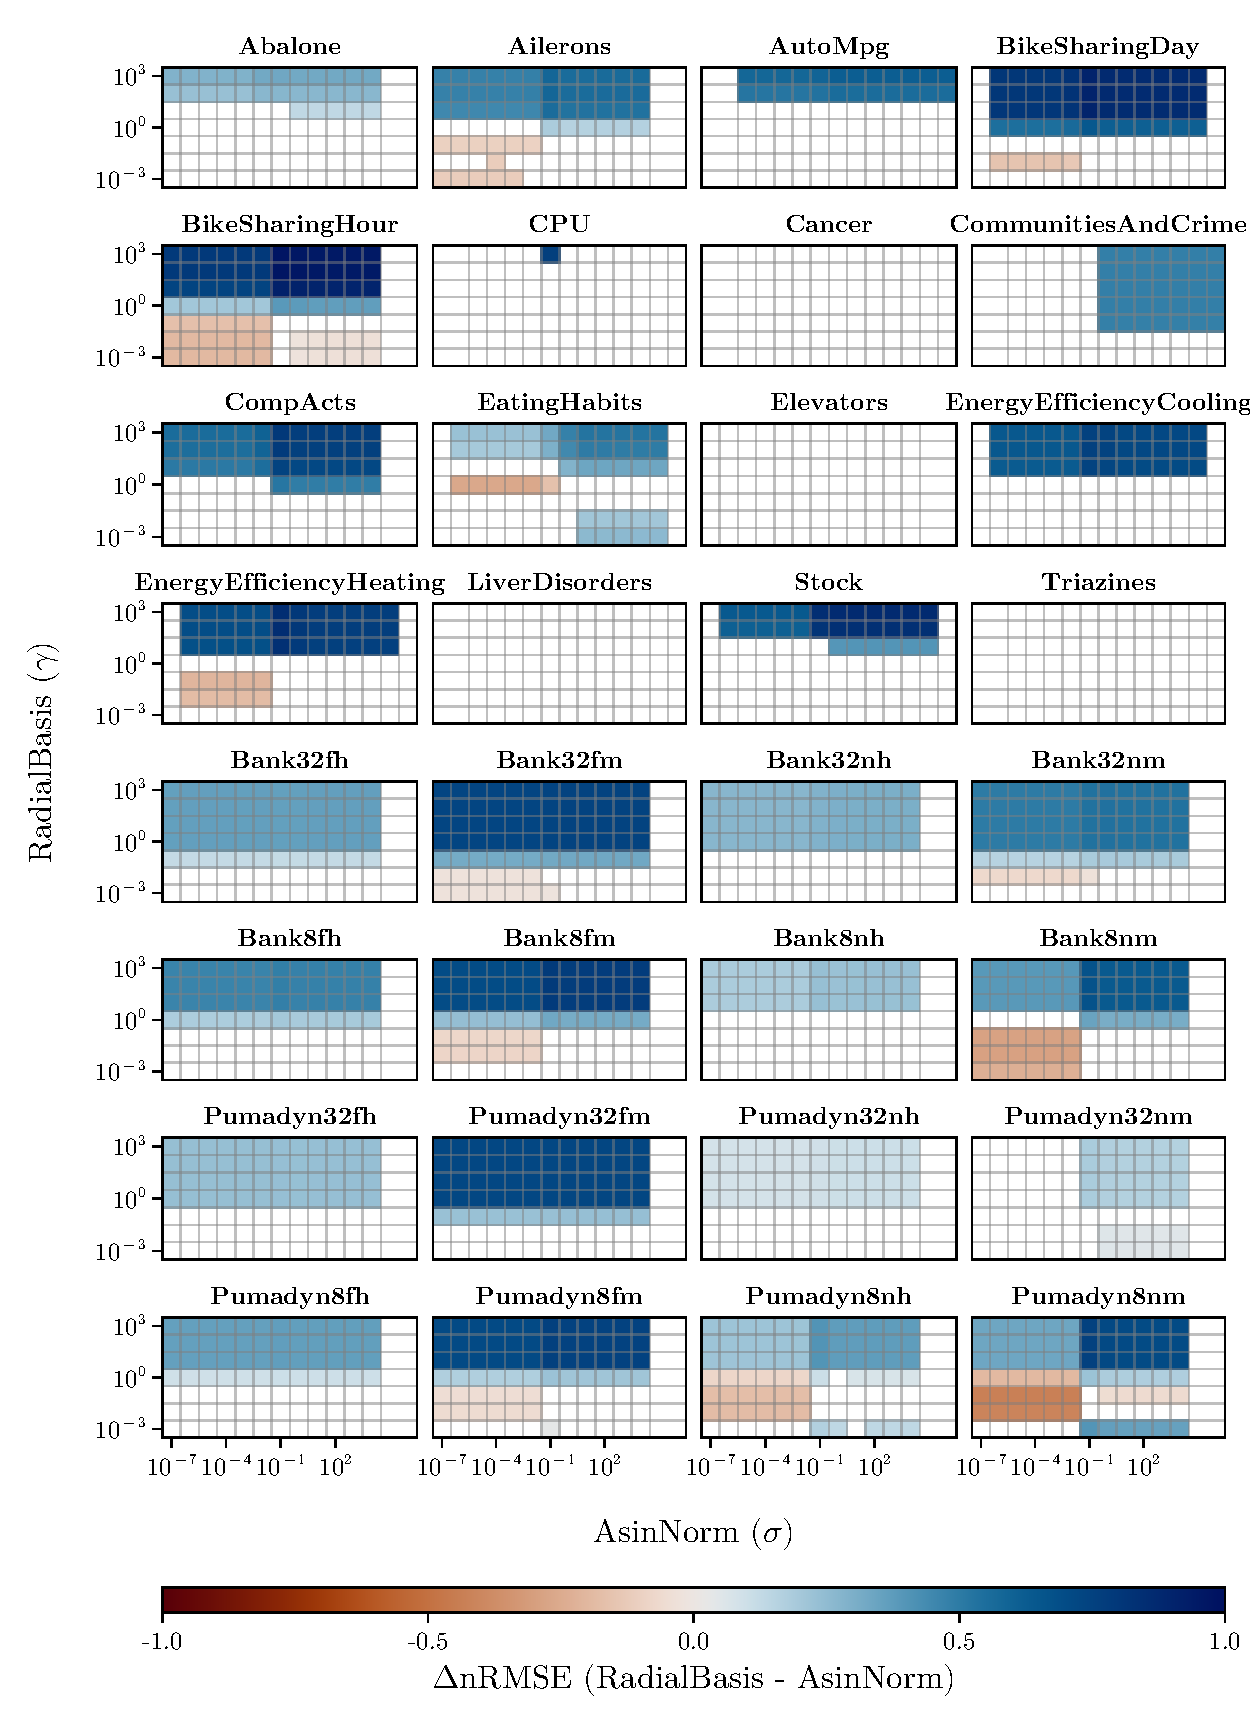
\includegraphics[width=0.9\textwidth]{plots/heatmaps_rbf_asinnorm_s}
    \caption{Difference between nRMSE of RBF and normalized arc-sine kernels}
    \label{fig:heatmaps-rbf-asinnorm}
\end{figure}

\Cref{fig:heatmaps-asin-asinnorm} shows the difference between the non normalized
and the normalized arc-sine kernels. Positive values indicate that the normalized
kernel performs better. We can see that the values in the top right corner (both sigmas $>1$)
of all the datasets is zero. Which indicates that they perform equally well.

\begin{figure}[H]
    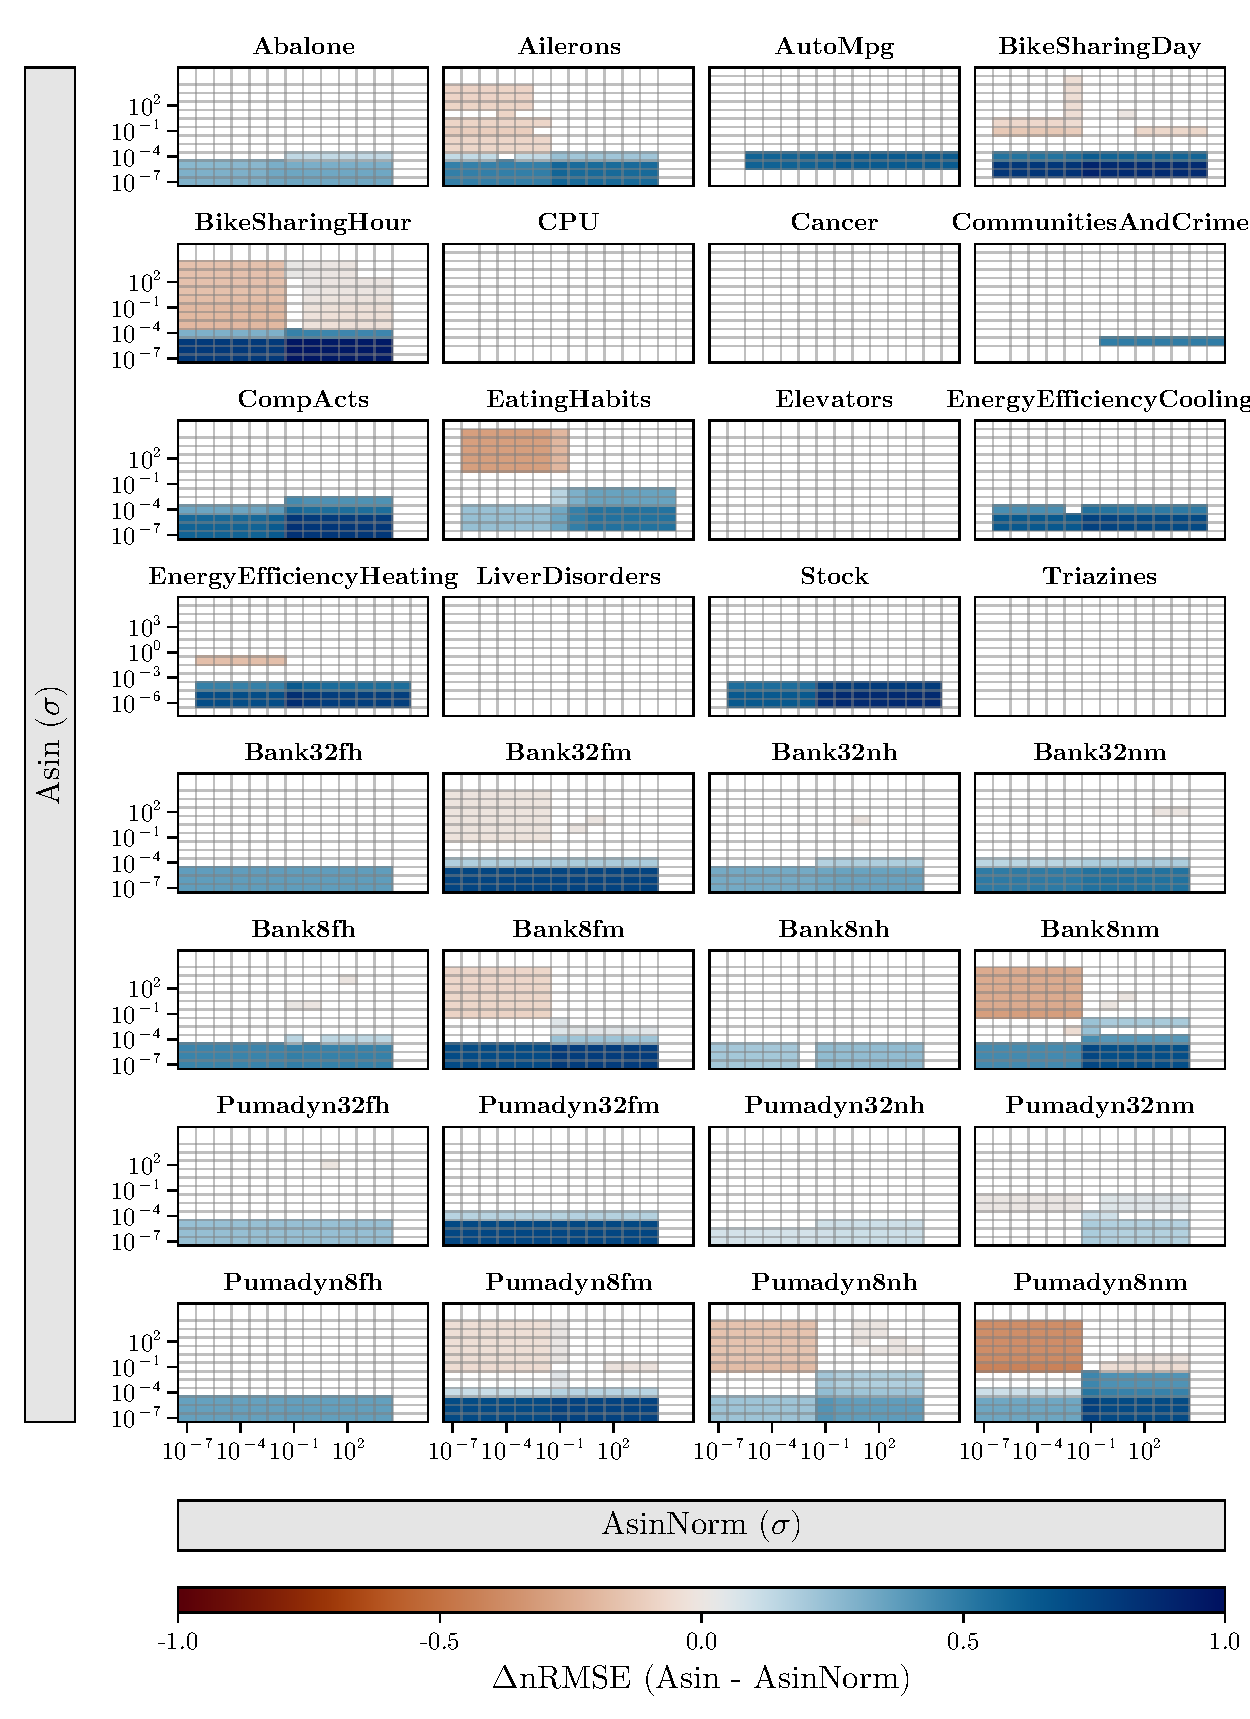
\includegraphics[width=0.9\textwidth]{plots/heatmaps_asin_asinnorm_s}
    \caption{Difference between nRMSE of arc-sine and normalized arc-sine kernels}
    \label{fig:heatmaps-asin-asinnorm}
\end{figure}

% TODO: maybe a combination plot of the heatmap and the line plot for some
% interesting datasets?

% TODO: classification is a mess
% \section{Classification}
%
% \begin{figure}[H]
%     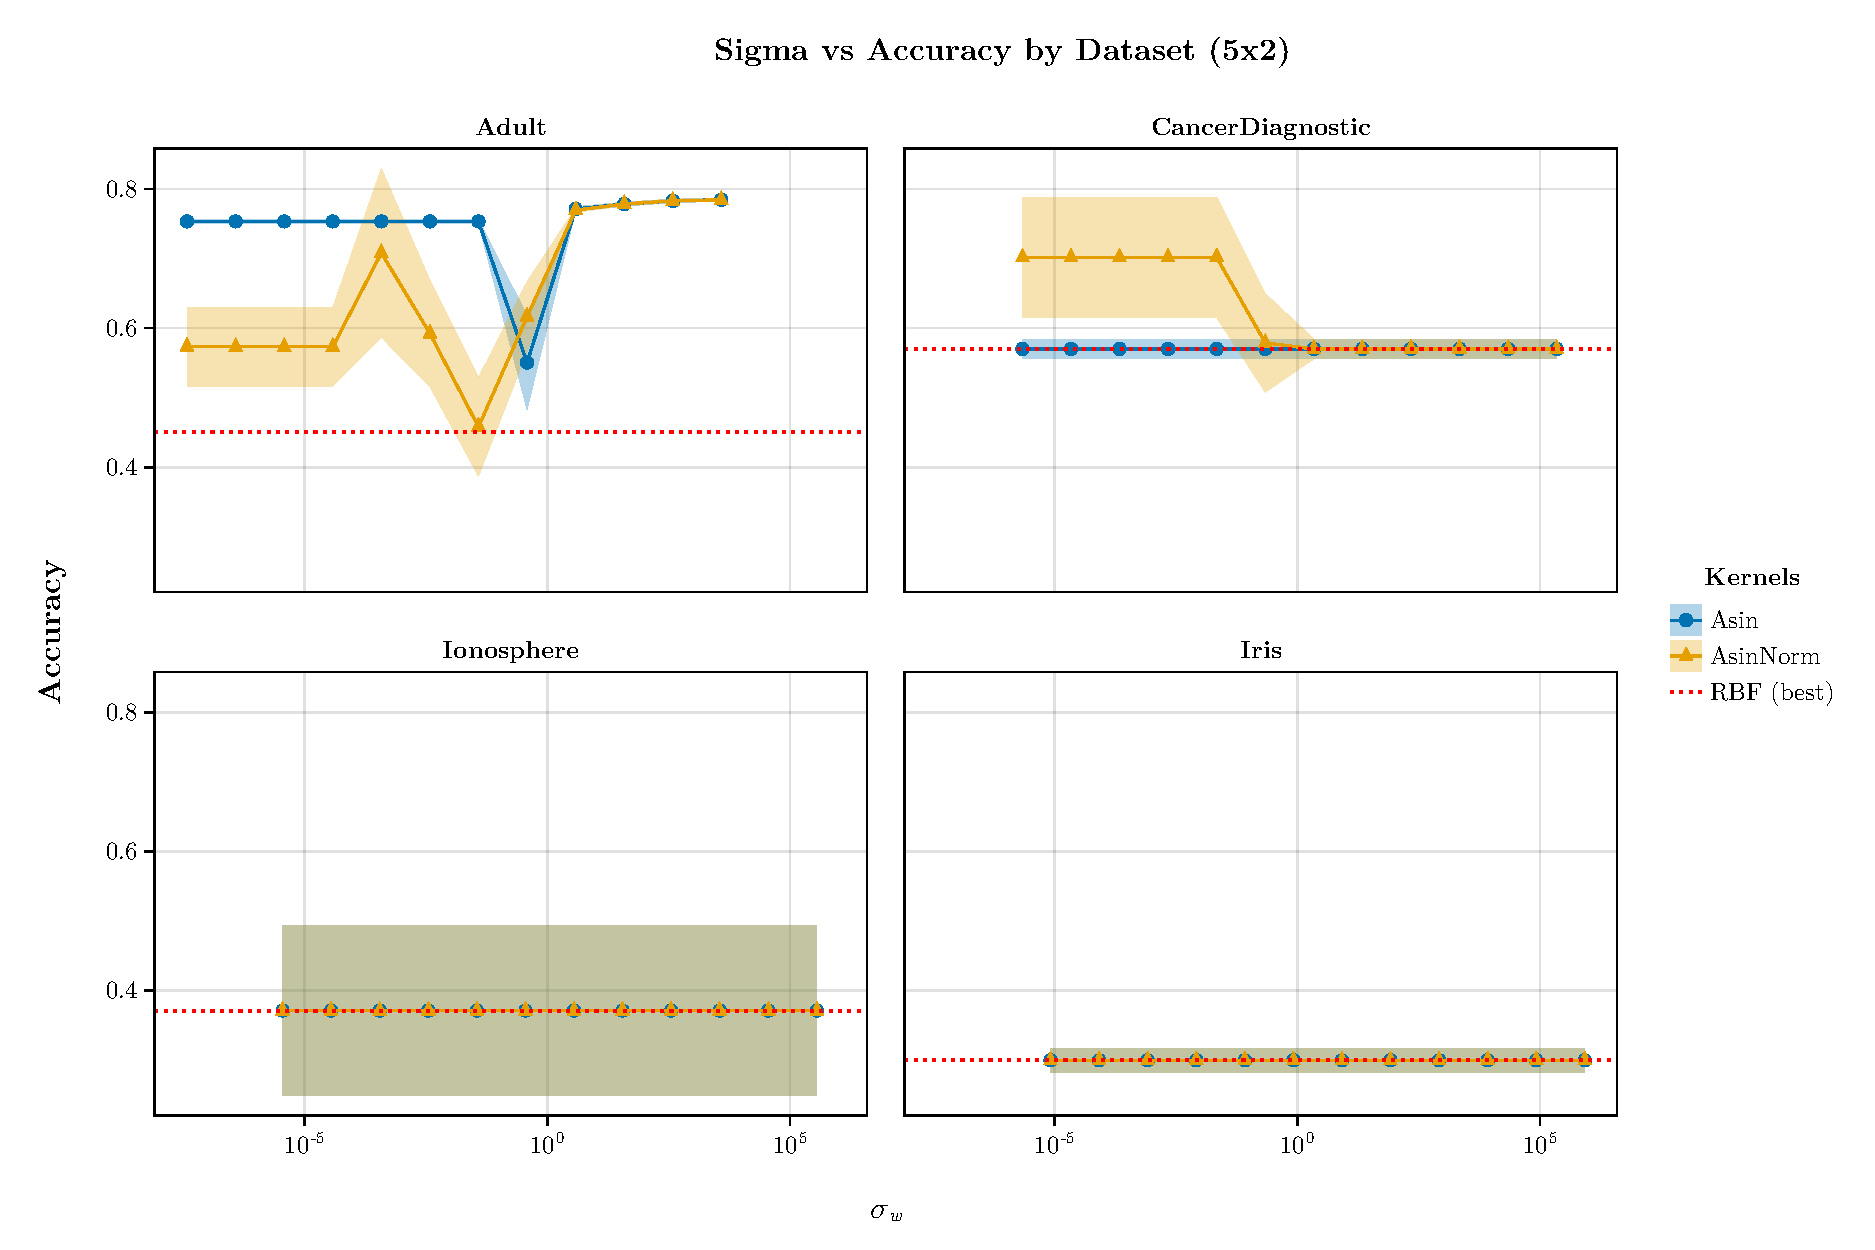
\includegraphics{plots/nRMSE_class_all_scaled}
%     \caption{Classification accuracy}
%     \label{fig:nrmse-class-all}
% \end{figure}
%
% \begin{marker}
%     This makes no sense, the accuracies are too low, specially iris (Even on the
%     RBF).
%
%     Add the other datasets.
%     Add more values of sigma.
%     Other metrics (precision, recall, f1, etc)
% \end{marker}

\section{Estimation of the time needed to train the SVM}

The main incentive for using the arc-sine kernel is that it is supposed to be
parameter insensitive, which means that we can reduce the search space for the
hyperparameters and thus reduce the time needed to train the SVM.

If for the RBF kernel we have to search for $n$ possible values of $\gamma$
hyperparameter whilst for the arc-sine kernel we can set $\sigma_w=10$ and
achieve similar results, then we can reduce the search space by a factor of $n$.

However, it is still possible that even with a fixed $\sigma_w$ the arc-sine
kernel requires a wider search space for the other hyperparameters (cost and
$\varepsilon$) or the computation of the kernel is more expensive than the RBF
and thus the time needed to train the SVM is not reduced.

For instance, in the initial testing of the normalized arc-sine kernel, the average
training for the Adult dataset using the normalized arc-sine kernel
took approximately 2 times longer than the RBF kernel.

% TODO: plots de temps de execucio
% TODO: plots de temps de iteracions / iteracions per segon
% TODO: plots de temps de nombre de parametres provats
%

\section{Meta-learning}

As explained in \cref{sec:meta-learning}, we want to use meta-learning
techniques to determine the best value of sigma for a given dataset, or at least
to determine if a dataset is a good candidate for the arc-sine kernel or not.
For that, we can create two models:
\begin{enumerate}
    \item Predict the best value of $\sigma_w$ for a given dataset.
    \item Predict whether a high value of $\sigma_w$ will achieve equivalent
          performance to the RBF kernel.
\end{enumerate}

For the first model,
we can use the best value of $\sigma_w$ for each dataset
obtained from the previous experiments. This will be our target
variable.

For the second model, we need to determine if there is a statistically
significant difference between the performance at $\sigma \gg 10$ and the
performance of the RBF kernel.
% TODO: t-test or arbitrary threshold?

% TODO: probably need a lot more datasets to be able to do anything...

\begin{note}
    With the number of datasets the results are not conclusive.
    Need much more datasets.
\end{note}

